\documentclass[titlepage]{article}

\usepackage[utf8]{inputenc}
\usepackage{scrextend}
\usepackage[bottom]{footmisc}
\usepackage{graphicx}
\usepackage{float}
\usepackage{listings}

\title{Comfy: Gestionnaire de fenêtres en tuile}
\author{Daniel-Junior Dubé et Félix Chabot}
\date{Session d'automne 2018}

\graphicspath{ {./images/} }

\lstset{frame=single,numbers=left,inputpath=./sources}

\begin{document}
\maketitle

\renewcommand{\contentsname}{Table des matières}
\tableofcontents
\newpage

\section{Introduction}
\par
\bigskip
Étant devenu depuis quelques années des enthousiastes des systèmes
d'exploi-tation GNU/Linux, nous avons pu observer l’engouement de la communauté
envers les gestionnaires des fenêtre en
tuile\footnote{https://en.wikipedia.org/w/index.php?title=Tiling\_window\_manager}.
En effet, ces gestionnaires permettent une plus grande flexibilité pour la
personnalisation de l’interface utilisateur que les environnements de bureau
populaire tel que \textit{Gnome}, \textit{KDE} et \textit{Xfce} tout en étant
plus léger sur l’utilisation des ressources matérielles. Tout comme les outils
minimalistes tel \textit{Vim} et \textit{Emacs}, ces gestionnaires de fenêtres
permettre aussi de bénéficier à l’efficacité des développeurs qui les utilisent
grâce aux fonctionnalités adaptées à ceux-ci.

\par
\bigskip
De plus, le tout nouveau protocole \textit{Wayland} commence à être adopté par
ces environnements de bureau. Il risque de remplacer le protocole \textit{X}
d'ici quelques années à cause de son architecture optimisée et pour sa
meilleure gestion des ressources matérielles.

\par
\bigskip
Nous avons donc décidé de concevoir un gestionnaire de fenêtres utilisant ce
nouveau protocole et qui sera écrit avec le langage de programmation
\textit{Rust}. Celui-ci est un langage apportant des fonctionnalités modernes
intéressantes en ce qui concerne la gestion mémoire et la concurrence, tout en
gardant une performance rivalisant celle du \textit{C} et \textit{C++}.  Il
existe peu de gestionnaires de fenêtres utilisant à la fois \textit{Rust} et
\textit{Wayland}. Il y en a un en particulier s’appelant
\textit{Way-Cooler}\footnote{http://way-cooler.org}, mais selon les auteurs de
ce projet, il n’est pas encore assez stable pour être utilisé en “production”.

\par
\bigskip
Notre but sera donc de créer un logiciel que des enthousiastes pourront
ultimement utiliser dans leur quotidien tout en nous permettant d’apprendre les
rudiments de la programmation de composantes systèmes.

\section{Revue de littérature}
\begin{description}
    \item [Écran] Un écran est un espace de rendu qui est mis à notre
        disposition par un appareil physique (moniteur).
    \item [Espace de travail] Un écran possède une liste d’espaces de travail.
        Un seul espace de travail est affiché à l’écran à la fois.
    \item [Disposition] Un espace de travail est constitué d’une seule
        disposition. Celle-ci est sous forme d’un arbre enraciné (k-ary tree),
        elle va déterminer la position et la
        dimension des fenêtres.
    \item [Noeud de disposition (dans l’arbre de disposition)] Noeud dans
        l’arbre de la disposition. Correspond essentiellement à un conteneur de
        fenêtres.
    \item [Subdivision] Une subdivision représente à la fois une entrée dans
        l’arbre de disposition et un sous-ensemble de l’espace d’affichage de
        l’écran.
    \item [Fenêtre] Une fenêtre est une feuille dans l’arbre de disposition.
        Elle est donc l’espace réservé à l’affichage du rendu d’une application
        en exécution.
    \item [Conteneur de fenêtres] Un conteneur est un noeud dans l’arbre de
        disposition. Il s’agit donc d’une structure de données qui va contenir
        un ensemble de fenêtres ou de
        conteneurs.
    \item [Gestionnaire de fenêtre] Un logiciel qui contrôle l’affichage et la
        disposition des fenêtres des applications en exécution.
    \item [Tuile] Correspond à l’espace (ou subdivision) de l’écran réservé à
        une fenêtre ou un conteneur de fenêtres.
\end{description}
	
\section{Diagrammes du fonctionnement}
\begin{figure}[H]
	\centering
	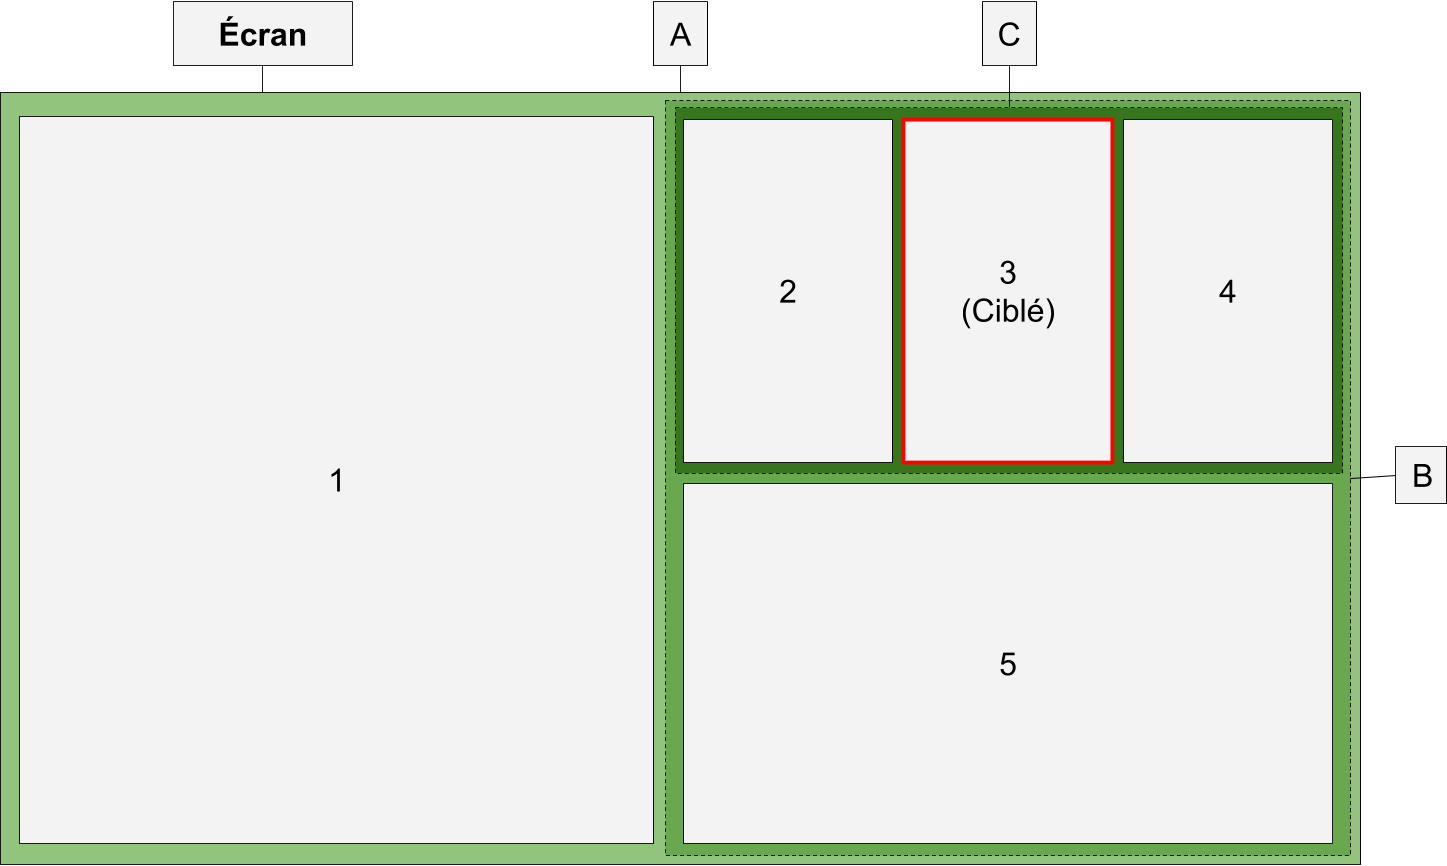
\includegraphics[width=\textwidth]{diagramme_du_fonctionnement.png}
	\caption{Représentation d'une intéraction normale de ces objets}
\end{figure}
\begin{figure}[H]
	\centering
	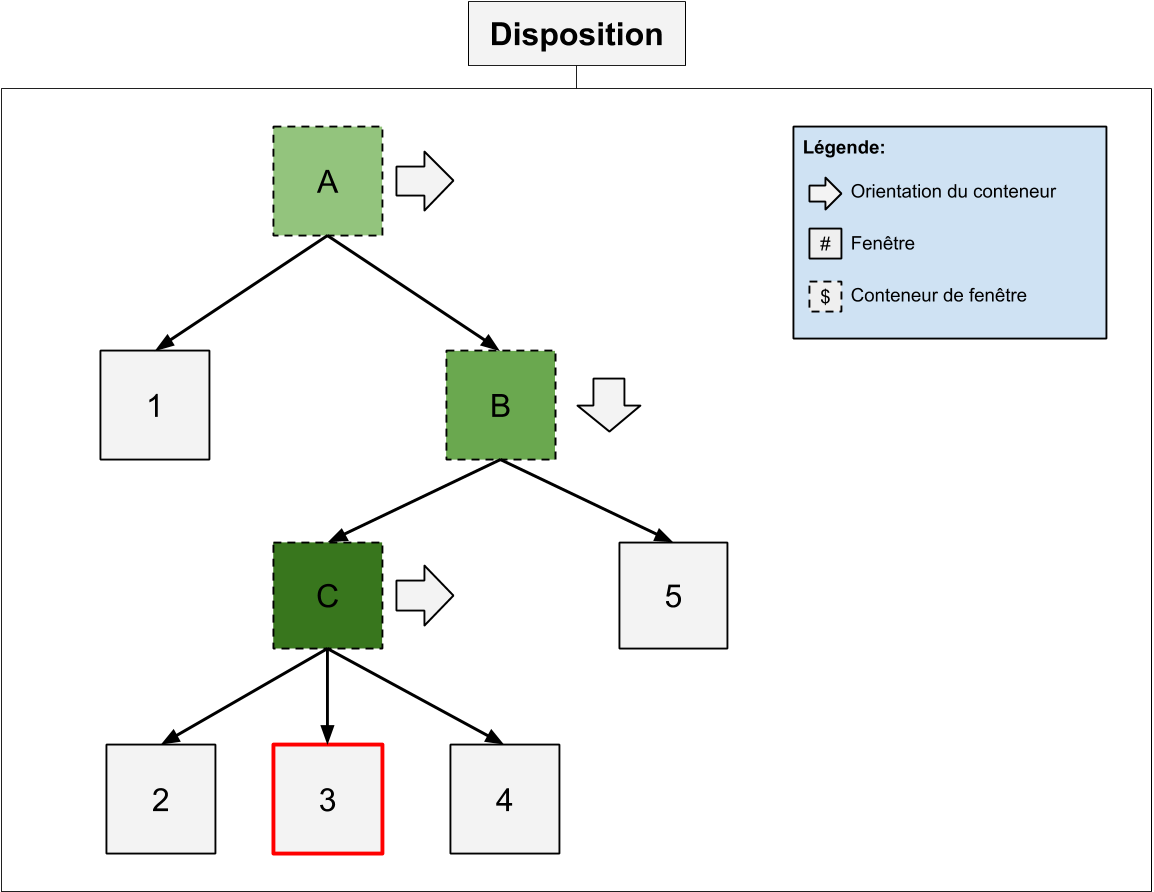
\includegraphics[width=\textwidth]{diagramme_du_fonctionnement_arbre.png}
	\caption{Arbre résultant}
\end{figure}
\section{Composantes}
\subsection{Configuration}

\par
\bigskip
Afin de donner une meilleure expérience aux utiliseurs de \textit{Comfy}, nous
avons décidé de laisser la possibilité de pouvoir personaliser un grand nombre
de fonctionnalités à même l'application. Le format des fichiers de
configuration sera en
\textit{TOML}\footnote{https://github.com/toml-lang/toml}. Ce format est
d'ailleurs utilisé pour les fichiers de configuration du langage \textit{Rust}.
\textit{TOML} est très similaire au \textit{JSON} pour la représentation des
différents types de données et de la simplicité d'écriture.  Par contre,
\textit{TOML} porte une plus grande importance à la lisibilité ce qui est un
point cruciale pour un fichier de configuration. De plus, il est possible de
rajouter des commentaires aux fichiers d'exemple ce qui va nous permettre de
bien expliquer les configurations possibles aux utilisateurs. Pour l'instant
nous prévoyons avoir deux fichiers de configurations:
\begin{itemize}
    \item Un fichier pour les raccourcis clavier appelé \textbf{keybings.toml}
    \item Un fichier pour l'apparence de comfy appelé \textbf{theme.toml}
\end{itemize}

\subsubsection{keybindings.toml}
\begin{minipage}{\linewidth}
    \lstinputlisting[label=keybindings-example,title=Exemple d'un fichier
    keybindings.toml]{keybindings.toml}
\end{minipage}

\par
Un paramètre important de notre fichier de configuration est \textit{modkey}
qui va servir à définir une sorte de macro qui va être utilisable tout au long
du fichier. Pour faire référence au \textit{modkey} il faut seulement entrer
\textit{\$mod} et \textit{Comfy} s'occupera de le remplacer à la bonne touche.
L'utilité du \textit{modkey} est de dédier de façon simple une touche centrale
de contrôle pour les commandes\footnote{Nous allons définir plus tard ce qu'est
une commande.} de \textit{Comfy}. Une touche parfaite pour le \textit{modkey}
serait une touche
modificatrice\footnote{https://fr.wikipedia.org/wiki/Touche\_de\_combinaison}
comme les touches \textbf{Control}, \textbf{Super} et \textbf{Alt} puisque
celles-ci ne devraient pas avoir un impact sur le fonctionnement des
applications sous-jacentes.
\par
\bigskip
Ensuite, nous avons la section \textbf{keybindings}. Cette section sera la
partie la plus importante du fichier puisque c'est dans celle-ci que nous
allons associer les combinaisons de touches à une commande. Une entrée de cette
section est relativement simple. Le membre gauche de l'égalité est un ensemble
de touches entre guillemets. Malheureusement, la clé en \textit{TOML} (qui est
le membre gauche en question) ne peut pas contenir de \textbf{+}, c'est
pourquoi nous utilisons les guillemets. Ensuite, le membre droit contient deux
parties, une commande suivie d'arguments. Par exemple, à la ligne 4 du fichier
d'exemple, nous avons:

\lstinputlisting[frame=none,numbers=none,firstline=4,lastline=4]{keybindings.toml}

La commande serait donc \textbf{exec} et l'argument serait
\textbf{weston-terminal}.

\par
\bigskip
Une chose importante à savoir est que \textit{Comfy} gère les entrées clavier
et vérifie si une combinaison de touches se trouve dans le fichier de
configuration et l'exécute. Ceci serait problématique si un raccourci serait
aussi associé dans une application. Par exemple, associer une commande à la
combinaison \textbf{Control+S} ne serait pas une bonne idée puisque celle-ci
sera toujours interceptée par \textit{Comfy} avant même de se rendre à
l'application.

\end{document}
